% Chapter 1: Introduction

\chapter{Introducción} % Main chapter title

\label{Chapter1}

%-------------------------------------------------------------------------------

% Define some commands to keep the formatting separated from the content
\newcommand{\keyword}[1]{\textbf{#1}}
\newcommand{\tabhead}[1]{\textbf{#1}}
\newcommand{\code}[1]{\texttt{#1}}
\newcommand{\file}[1]{\texttt{\bfseries#1}}
\newcommand{\option}[1]{\texttt{\itshape#1}}
\newcommand{\Mod}[1]{\ (\mathrm{mod}\ #1)}

%-------------------------------------------------------------------------------
En este capítulo se introduce el tema a tratar partiendo de conceptos previos que ayudarán al lector a entender mejor el desarrollo, siguiendo con la definición del problema y la motivación del mismo, y por último, se muestra una revisión del estado del arte relacionado con este problema.

\section{Estructura de la memoria}
La memoria de este trabajo final de grado se estructura de la siguiente manera:
\begin{itemize}
	\item Capítulo 1, en este capítulo se introduce el tema a tratar, describiendo el problema y el estado del arte del mismo, así como conceptos previos a tener en cuenta.
	\item Capítulo 2, en este capítulo se muestran los objetivos que se esperan alcanzar con este trabajo final de grado.
	\item Capítulo 3, en este capítulo se describe de manera algorítmica la metaheurística empleada para abordar el problema tratado.
	\item Capítulo 4, en este capítulo se explica el desarrollo de las funciones para obtener una solución al problema.
	\item Capítulo 5, en este capítulo se exponen los resultados recopilados durante el procesamiento del problema, así como el análisis de los mismos.
	\item Capítulo 6, en este capítulo se muestran las conclusiones finales obtenidas durante todo este trabajo final de grado.
\end{itemize}

\section{Conceptos previos}
Para comprender mejor todas las explicaciones que se van a exponer a lo largo de toda esta memoria, se van a describir algunos conceptos a continuación.

\subsection{Optimización combinatoria}
aaa

\subsection{Heurística y Metaheurística}
Se define heurística, según el Diccionario de la Real Academia de la Lengua Española \cite{rae-heuristica}, como ``técnica de la indagación y del descubrimiento'' y ``en algunas ciencias, manera de buscar la solución de un problema mediante métodos no rigurosos, como por tanteo, reglas empíricas, etc.''.

Aplicándolo a temas científicos se define como el proceso de creación de medios, estrategias y principios para alcanzar un objetivo eficaz al problema dado \cite{conceptodef-heuristica}, y en relación a esto, el término, fue acuñado por George Polya en su libro ``How to Solve It'' \cite{gpolya-book-1}, más tarde traducido a ``Cómo plantear y resolver problemas'' \cite{gpolya-book-2}.

Añadiendo al término heurística el prefijo ``meta'' procedente del griego, que significa ``más allá'' o ``nivel superior'', se puede definir metaheurística como el conjunto de procedimientos heurísticos combinados para obtener una solución, aunque no exacta si eficiente, a un problema que no tiene un algoritmo heurístico específico o su aplicación es ineficiente \cite{wiki-metaheuristica}. Este término lo acuño Fred Glover en sus trabajos sobre búsqueda tabú en 1986 \cite{fred-glover}.

Existen un gran variedad de algoritmo metaheurísticos que se pueden clasificar de diferentes maneras según el enfoque, en la figura \ref{fig:clasif-metahs} se muestra una de ellas basada en el número de soluciones.\\
\begin{figure}[H]
	\centering
	\diagram{Trayectoriales}{
		- \diagram{Búsqueda\\local}{
			- Con memoria: Búsqueda Tabú (\gls{TS})\\ 
			- \diagram{Estocástica}{
				- Búsqueda local guiada (\gls{GLS}) \\ 
				- Métodos ruidosos (\gls{NM}) \\ 
				- Recocido simulado (\gls{SA})\\
				- Métodos de aceptación de\\ umbral (\gls{TAM})\\
			}\\
			- \diagram{Por \\entornos}{
				- Búsqueda de entorno variable (\gls{VNS})\\
				- Optimización parcial bajo condiciones\\ especiales de intensificación(\gls{POPMUSIC})\\
			}\\
		}\\
		- \diagram{Búsqueda\\iterativa}{
			- Búsqueda local iterativa (\gls{ILS})\\
			- Búsqueda por entorno adaptativo borroso (\gls{FANS})\\
		}\\
		- \diagram{Búsqueda\\multi-arranque}{
			- Concentración heurística (\gls{HC})\\
			- Métodos multi-arranque adaptativos (\gls{AMS})\\
			- Métodos multi-arranque (\gls{MSM})\\
			- Procedimientos de búsqueda voráz,\\ aleatorizada y adaptativa (\gls{GRASP})\\
		}\\
	}
	\diagram{Poblacionales}{
		- \diagram{Combinación\\de soluciones}{
			- \diagram{Inspiración\\evolutiva}{
				- Algoritmos culturales (\gls{CA})\\
				- Algoritmos genéticos (\gls{GA})\\
				- Algoritmos meméticos (\gls{MA})\\
			}\\
			- \diagram{Sin inspiración}{
				- Re-encadenamiento de\\ caminos (\gls{PR})\\
				- Búsqueda dispersa (\gls{SS})\\
			}\\
		}\\
		- \diagram{Movimientos}{
			- Optimización por colonias de hormigas (\gls{ACO})\\
			- Equipos asíncronos (\gls{AT})\\
			- Algoritmos de estimación de distribución (\gls{EDA})\\
			- Inteligencia de enjambre (\gls{SI})\\
		}\\
	}
	\caption{Clasificación de metaheurísticas}
	\label{fig:clasif-metahs}
\end{figure}

Dos conceptos a tener en cuenta en un algoritmo metaheurístico son la intensificación o explotación en una región, de modo que una alta intensificación hará que el algoritmo realice una búsqueda más exhaustiva en esa región, y la diversificación o exploración de nuevas regiones del espacio de soluciones \cite{libro-metaheuristicas}.

\subsection{Clique}
\label{sec-clique}
El término clique se puede asemejar a un grupo de personas, las cuales serían los nodos o vértices de un grafo, a las que les unen los mismos intereses por algún tema en concreto, estas uniones serían las aristas que unen los nodos del grafo \cite{LUCE:1949}.

En teoría de grafos, un clique, es el subgrafo, perteneciente a un grafo, en el cuál todos sus nodos o vértices son adyacentes entre sí, es decir, todo par de nodos o vértices está conectados mediante una arista, en términos matemáticos se describe como, dado un grafo $G = (V, E)$ donde $V$ indica el conjunto de vértices del grafo y $E$ indica el conjunto de aristas del grafo \cite{web-clique}, un clique se define como:
\[
C \subseteq V(G) ~ \wedge ~ u, v ~ \epsilon ~ C  \wedge  u  \neq v \Rightarrow u, v ~ \epsilon ~ E(G)
\]

\begin{figure}[H]
	\centering
	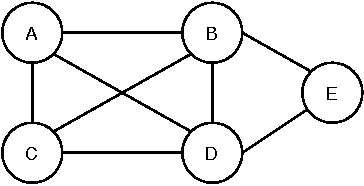
\includegraphics{Figures/graph.pdf}
	\caption{Diagrama de un grafo.}
	\label{fig:graph}
\end{figure}

En la figura \ref{fig:graph} se muestra un grafo compuesto por el conjunto de nodos \\$V=\{A, B, C, D, E\}$, en este grafo se encuentran como indican las figuras \ref{fig:graph-cliques-2} y \ref{fig:graph-cliques-3} los posibles cliques de este grafo, donde $k$ indica el número de nodos del clique. Cabe resaltar, que los nodos por si solos también forman clique, pero no se ha incluido para no hacer más compleja la figura.

\begin{figure}[H]
	\centering	
	\subfigure[Clique A-B]{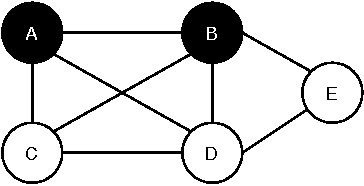
\includegraphics[width=0.275\textwidth]{Figures/graph-clique-AB.pdf}}
	\subfigure[Clique A-C]{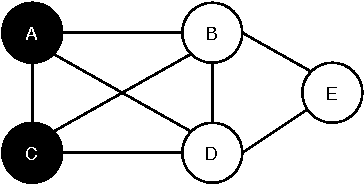
\includegraphics[width=0.275\textwidth]{Figures/graph-clique-AC.pdf}}
	\subfigure[Clique A-D]{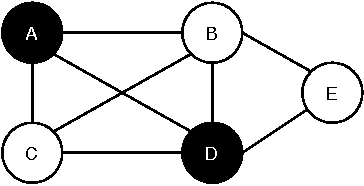
\includegraphics[width=0.275\textwidth]{Figures/graph-clique-AD.pdf}}
	\subfigure[Clique B-C]{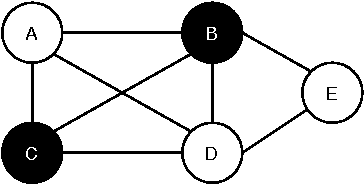
\includegraphics[width=0.275\textwidth]{Figures/graph-clique-BC.pdf}}
	\subfigure[Clique B-D]{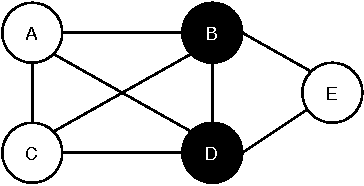
\includegraphics[width=0.275\textwidth]{Figures/graph-clique-BD.pdf}}
	\subfigure[Clique B-E]{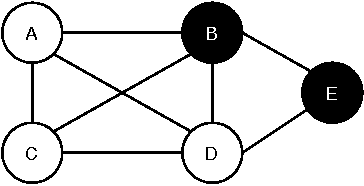
\includegraphics[width=0.275\textwidth]{Figures/graph-clique-BE.pdf}}
	\subfigure[Clique C-D]{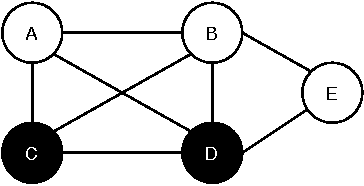
\includegraphics[width=0.275\textwidth]{Figures/graph-clique-CD.pdf}}
	\subfigure[Clique D-E]{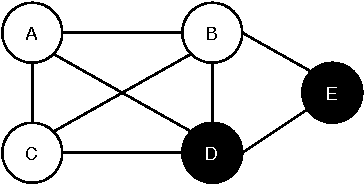
\includegraphics[width=0.275\textwidth]{Figures/graph-clique-DE.pdf}}
	\caption{Cliques $k$ = 2 del grafo.}
	\label{fig:graph-cliques-2}
\end{figure}

\begin{figure}[H]
	\centering	
	\subfigure[Clique A-B-C]{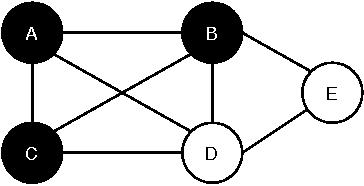
\includegraphics[width=0.275\textwidth]{Figures/graph-clique-ABC.pdf}}
	\subfigure[Clique A-B-D]{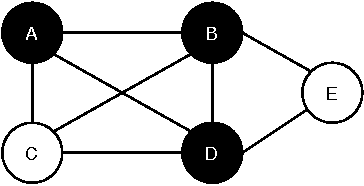
\includegraphics[width=0.275\textwidth]{Figures/graph-clique-ABD.pdf}}
	\subfigure[Clique A-C-D]{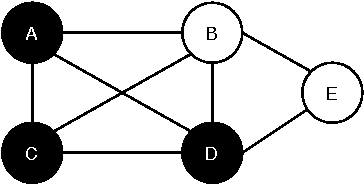
\includegraphics[width=0.275\textwidth]{Figures/graph-clique-ACD.pdf}}
	\subfigure[Clique B-C-D]{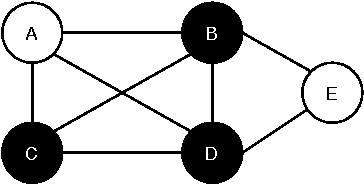
\includegraphics[width=0.275\textwidth]{Figures/graph-clique-BCD.pdf}}
	\subfigure[Clique B-D-E]{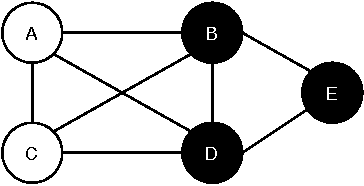
\includegraphics[width=0.275\textwidth]{Figures/graph-clique-BDE.pdf}}
	\caption{Cliques $k$ = 3 del grafo.}
	\label{fig:graph-cliques-3}
\end{figure}

Es importante resaltar que un clique perteneciente a un grafo, no implica que sea máximo, puesto que un clique máximo es el clique el cuál no es posible ampliar, es decir, no se pueden añadir a este más adyacentes que cumplan con las restricciones necesarias para formar un clique y a su vez es el de mayor tamaño del grafo, como se muestra en la figura \ref{fig:max-clique}, a diferencia de un clique que se podría denominar simple  \cite{web-maximalclique}\cite{web-maximumclique}. Y en este  caso, se obtiene que:
\[
\omega(G) = 4
\]
donde $\omega$ denota el número de vértices del clique, su cardinalidad.
\begin{figure}[H]
	\centering
	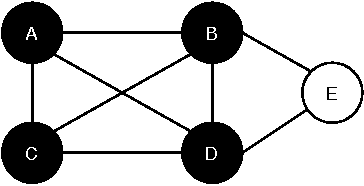
\includegraphics{Figures/graph-clique-max.pdf}
	\caption{Clique máximo del grafo.}
	\label{fig:max-clique}
\end{figure}

\section{Definición y motivación del problema}

\subsection{Problema del clique de ratio máximo}
\label{intro-problema}
Como se introdujo en la sección \ref{sec-clique} el concepto clique en cuanto a teoría de grafos es fundamental y muy estudiado, y más concretamente la búsqueda del clique máximo dentro de un grafo, a este problema se le conoce como ``El problema del clique máximo'' o \gls{MCP} por sus siglas en ingles ``Maximum clique problem'', y es catalogado como un problema NP-completo, como se aprecia en la figura \ref{fig:problemas-np}.

\begin{figure}[H]
	\centering
	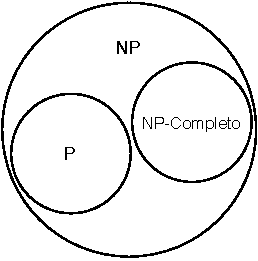
\includegraphics{Figures/problemas-np.pdf}
	\caption{Diagrama de problemas NP.}
	\label{fig:problemas-np}
\end{figure}

Los problemas denominados como NP, acrónimo de non-deterministic polynomial time o tiempo polinominal no determinista, en teoría de complejidad computacional, se les conoce como el conjunto de problemas que se pueden resolver en un tiempo polinómico por una máquina de Turing no determinista. Esta clasificación, además, contiene todos los problemas de tipo P y de tipo NP-completos como es el caso del problema del clique máximo.

Una variante de este problema es el llamado ``Problema de clique de peso máximo'' o \gls{MWCP} por sus siglas en inglés a Maximum weight clique problem, en el que se asocia un peso no negativo a cada vértice y cuyo objetivo es encontrar un clique con el máximo valor en la suma de los pesos de sus vértices. Este problema esta estrechamente ligado al problema tratado en este trabajo final de grado, el cual busca el clique de ratio máximo ya que si se asocian dos pesos no negativos a cada vértice se obtiene el problema del clique de ratio máximo \gls{MRCP} o ``Maximum Ratio Clique Problem''. En este problema se busca el clique máximo en un grafo con la mayor proporción de ratio. Esta proporción se define como las sumas de los pesos de los vértices.

\begin{equation*}
\frac{\sum_{i=1}^{n}p_ix_i}{\sum_{i=1}^{n}q_ix_i}
\end{equation*}

donde $p$ y $q$ son pesos no negativos asociados a cada vértice $i$, y $x$ se determina como:
\[
\diagram{$x_i=$}{
	1 : si el vértice $i$ forma parte del clique solución. \\
	0 : en otro caso
}
\]

Por lo tanto, el objetivo del problema es maximizar esta proporción como se expone en el modelo de ecuación \ref{eq:mrcp-max}, partiendo de un grafo simple no dirigido $G=(V, E)$, donde $V$ se asocia al conjunto de vértices pertenecientes al grafo, $\{v_1,\dots,v_n\}$, y $E$ es el conjunto de aristas que conectan los vértices del grafo, $\{v_i,~v_j\}$ tal que $i \neq j$ y $v_i,~v_j~\in V$, y suponiendo que los pesos asociados a cada vértice son positivos, se obtiene un clique máximo $\widehat{S}$, siempre y cuando se cumplan las restricciones \ref{eq:mrcp-rest1} - \ref{eq:mrcp-rest3}.

\begin{eqnarray}
\label{eq:mrcp-max} 
maximizar && f = \frac{\sum_{i=1}^{n}p_ix_i}{\sum_{i=1}^{n}q_ix_i} \\
\nonumber sujeto ~ a: \\
\label{eq:mrcp-rest1}
&& x_i + x_j \leqslant 1 : \forall (v_i, v_j) \notin E,~i \neq j,\\
\label{eq:mrcp-rest2}
&& \sum_{i=1}^{n}(a_ij)x_i ~ \geqslant 1 : \forall v_j \in V, \\
\label{eq:mrcp-rest3}
&& x_i \in {0,~1} : \forall v_i \in V.
\end{eqnarray}

El problema del clique de ratio máximo ha sido catalogado como un problema NP-difícil o NP-complejo, como se aprecia en la figura \ref{fig:np-dificil}, por lo que no es posible obtener una solución factible por métodos heurísticos o exactos.

\begin{figure}[H]
	\centering
	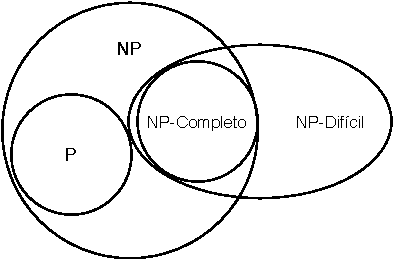
\includegraphics{Figures/problemas-np-hard.pdf}
	\caption{Diagrama de problemas Np y NP-difícil.}
	\label{fig:np-dificil}
\end{figure}

\subsection{Motivación del problema}

aaaaa

\section{Estado del arte}
El análisis sobre el estado del arte que se ha realizado sobre el problema del clique de ratio máximo y todo lo que rodea al mismo 

Moeini dca

\cite{mrcp-ants}

\cite{mrcp-Sethuraman:2015}

Cabe destacar entre todos los trabajos realizados sobre el problema del clique de ratio máximo el de Dominik Goeke, Mahdi Moeini y David Poganiuch \cite{mrcp-GOEKE2017283} el cuál se ha tomado como referencia para realizar este trabajo final de grado.

%-------------------------------------------------------------------------------

